\coverchapter{Strategies for TileScope}\label{ch:strats}
This chapter introduces three new strategies for TileScope, column reverse, column permutation and sliding. The first two, although perfectly valid strategies on their own, are used to extend sliding to any columns. The sliding strategy, as previously mentioned, allowed for the first discovery of a specification for $\Av{1432}$ by TileScope. 

Using a specification for $\Av{1234}$ discovered by TileScope and applying the same strategies at every step starting with $\Av{1432}$, we had a matching tree except for one tiling that we failed to expand in the same manner as the one for $\Av{1234}$. By looking at the tree we had created from the $\Av{1432}$ root, we could see what tiling was needed instead of the one we failed to expand in order to complete the specification in the same way. This pair of tilings, shown in \FigureRef{fig:slidepair}, whose inconspicuous equivalence we failed to disprove, is the motivation for the sliding strategy. The process of applying the same strategies to another root further motivated the automated bijection search in Chapters \ref{ch:parallel}, \ref{ch:pbijection} and \ref{ch:search}.

\begin{figure}[ht!]
    \centering
    \begin{center}
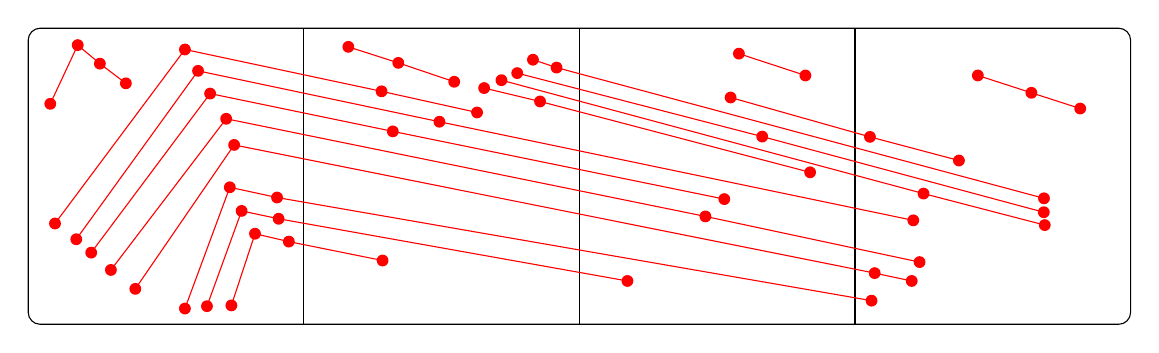
\begin{tikzpicture}[scale=1, every node/.style={scale=1}]
        \def\xscale{1.0} % Horizontal scale factor
        \def\yscale{1.0} % Vertical scale factor
        \def\spnt{0.075} % Size of smaller points
        \def\lpnt{0.125} % Size of larger points
        \def\roundscale{0.5} % The rounding factor
        \draw[rounded corners=2ex*\roundscale] (0,0) rectangle (14.0*\xscale,3.76*\yscale);
        \draw (3.5*\xscale, 3.76*\yscale) -- (3.5*\xscale, 0);
        \draw (7.0*\xscale, 3.76*\yscale) -- (7.0*\xscale, 0);
        \draw (10.5*\xscale, 3.76*\yscale) -- (10.5*\xscale, 0);
        \fill[red] (9.025415261218319*\xscale, 3.4370300409410106*\yscale) circle (\spnt);
        \fill[red] (9.87*\xscale, 3.16*\yscale) circle (\spnt);
        \draw[red] (9.025415261218319*\xscale, 3.4370300409410106*\yscale) -- (9.87*\xscale,3.16*\yscale);
        \fill[red] (4.065389790651616*\xscale, 3.523465393533877*\yscale) circle (\spnt);
        \fill[red] (4.7*\xscale, 3.32*\yscale) circle (\spnt);
        \fill[red] (5.41*\xscale, 3.08*\yscale) circle (\spnt);
        \draw[red] (4.065389790651616*\xscale, 3.523465393533877*\yscale) -- (4.7*\xscale,3.32*\yscale) -- (5.41*\xscale,3.08*\yscale);
        \fill[red] (5.79*\xscale, 3.0*\yscale) circle (\spnt);
        \fill[red] (6.5*\xscale, 2.83*\yscale) circle (\spnt);
        \fill[red] (9.93*\xscale, 1.93*\yscale) circle (\spnt);
        \draw[red] (5.79*\xscale, 3.0*\yscale) -- (6.5*\xscale,2.83*\yscale) -- (9.93*\xscale,1.93*\yscale);
        \fill[red] (6.41*\xscale, 3.36*\yscale) circle (\spnt);
        \fill[red] (6.71*\xscale, 3.26*\yscale) circle (\spnt);
        \fill[red] (12.9*\xscale, 1.6*\yscale) circle (\spnt);
        \draw[red] (6.41*\xscale, 3.36*\yscale) -- (6.71*\xscale,3.26*\yscale) -- (12.9*\xscale,1.6*\yscale);
        \fill[red] (6.21*\xscale, 3.19*\yscale) circle (\spnt);
        \fill[red] (9.32171125483173*\xscale, 2.383876554253752*\yscale) circle (\spnt);
        \fill[red] (12.897616736321888*\xscale, 1.4229999446867156*\yscale) circle (\spnt);
        \draw[red] (6.21*\xscale, 3.19*\yscale) -- (9.32171125483173*\xscale,2.383876554253752*\yscale) -- (12.897616736321888*\xscale,1.4229999446867156*\yscale);
        \fill[red] (6.01*\xscale, 3.1*\yscale) circle (\spnt);
        \fill[red] (11.37*\xscale, 1.66*\yscale) circle (\spnt);
        \fill[red] (12.91*\xscale, 1.26*\yscale) circle (\spnt);
        \draw[red] (6.01*\xscale, 3.1*\yscale) -- (11.37*\xscale,1.66*\yscale) -- (12.91*\xscale,1.26*\yscale);
        \fill[red] (8.92*\xscale, 2.88*\yscale) circle (\spnt);
        \fill[red] (10.69*\xscale, 2.38*\yscale) circle (\spnt);
        \fill[red] (11.82*\xscale, 2.08*\yscale) circle (\spnt);
        \draw[red] (8.92*\xscale, 2.88*\yscale) -- (10.69*\xscale,2.38*\yscale) -- (11.82*\xscale,2.08*\yscale);
        \fill[red] (12.06*\xscale, 3.16*\yscale) circle (\spnt);
        \fill[red] (12.74*\xscale, 2.94*\yscale) circle (\spnt);
        \fill[red] (13.36*\xscale, 2.74*\yscale) circle (\spnt);
        \draw[red] (12.06*\xscale, 3.16*\yscale) -- (12.74*\xscale,2.94*\yscale) -- (13.36*\xscale,2.74*\yscale);
        \fill[red] (0.28*\xscale, 2.8*\yscale) circle (\spnt);
        \fill[red] (0.6286433582040536*\xscale, 3.545653104388464*\yscale) circle (\spnt);
        \fill[red] (0.91*\xscale, 3.31*\yscale) circle (\spnt);
        \fill[red] (1.24*\xscale, 3.06*\yscale) circle (\spnt);
        \draw[red] (0.28*\xscale, 2.8*\yscale) -- (0.6286433582040536*\xscale,3.545653104388464*\yscale) -- (0.91*\xscale,3.31*\yscale) -- (1.24*\xscale,3.06*\yscale);
        \fill[red] (2.58*\xscale, 0.24*\yscale) circle (\spnt);
        \fill[red] (2.88*\xscale, 1.15*\yscale) circle (\spnt);
        \fill[red] (3.31*\xscale, 1.05*\yscale) circle (\spnt);
        \fill[red] (4.5*\xscale, 0.81*\yscale) circle (\spnt);
        \draw[red] (2.58*\xscale, 0.24*\yscale) -- (2.88*\xscale,1.15*\yscale) -- (3.31*\xscale,1.05*\yscale) -- (4.5*\xscale,0.81*\yscale);
        \fill[red] (2.27*\xscale, 0.23*\yscale) circle (\spnt);
        \fill[red] (2.71*\xscale, 1.44*\yscale) circle (\spnt);
        \fill[red] (3.18*\xscale, 1.34*\yscale) circle (\spnt);
        \fill[red] (7.61*\xscale, 0.55*\yscale) circle (\spnt);
        \draw[red] (2.27*\xscale, 0.23*\yscale) -- (2.71*\xscale,1.44*\yscale) -- (3.18*\xscale,1.34*\yscale) -- (7.61*\xscale,0.55*\yscale);
        \fill[red] (1.99*\xscale, 0.2*\yscale) circle (\spnt);
        \fill[red] (2.56*\xscale, 1.74*\yscale) circle (\spnt);
        \fill[red] (3.16*\xscale, 1.61*\yscale) circle (\spnt);
        \fill[red] (10.71*\xscale, 0.3*\yscale) circle (\spnt);
        \draw[red] (1.99*\xscale, 0.2*\yscale) -- (2.56*\xscale,1.74*\yscale) -- (3.16*\xscale,1.61*\yscale) -- (10.71*\xscale,0.3*\yscale);
        \fill[red] (0.34*\xscale, 1.28*\yscale) circle (\spnt);
        \fill[red] (1.99*\xscale, 3.49*\yscale) circle (\spnt);
        \fill[red] (4.487393024959084*\xscale, 2.958642977916958*\yscale) circle (\spnt);
        \fill[red] (5.7*\xscale, 2.69*\yscale) circle (\spnt);
        \draw[red] (0.34*\xscale, 1.28*\yscale) -- (1.99*\xscale,3.49*\yscale) -- (4.487393024959084*\xscale,2.958642977916958*\yscale) -- (5.7*\xscale,2.69*\yscale);
        \fill[red] (0.8*\xscale, 0.91*\yscale) circle (\spnt);
        \fill[red] (2.31*\xscale, 2.93*\yscale) circle (\spnt);
        \fill[red] (4.63*\xscale, 2.45*\yscale) circle (\spnt);
        \fill[red] (8.84*\xscale, 1.59*\yscale) circle (\spnt);
        \draw[red] (0.8*\xscale, 0.91*\yscale) -- (2.31*\xscale,2.93*\yscale) -- (4.63*\xscale,2.45*\yscale) -- (8.84*\xscale,1.59*\yscale);
        \fill[red] (0.61*\xscale, 1.08*\yscale) circle (\spnt);
        \fill[red] (2.1566952483766944*\xscale, 3.218645736093965*\yscale) circle (\spnt);
        \fill[red] (5.222205855724229*\xscale, 2.5723906205811886*\yscale) circle (\spnt);
        \fill[red] (11.24*\xscale, 1.32*\yscale) circle (\spnt);
        \draw[red] (0.61*\xscale, 1.08*\yscale) -- (2.1566952483766944*\xscale,3.218645736093965*\yscale) -- (5.222205855724229*\xscale,2.5723906205811886*\yscale) -- (11.24*\xscale,1.32*\yscale);
        \fill[red] (1.05*\xscale, 0.69*\yscale) circle (\spnt);
        \fill[red] (2.5140566365004244*\xscale, 2.6099847688049023*\yscale) circle (\spnt);
        \fill[red] (8.6*\xscale, 1.37*\yscale) circle (\spnt);
        \fill[red] (11.32*\xscale, 0.79*\yscale) circle (\spnt);
        \draw[red] (1.05*\xscale, 0.69*\yscale) -- (2.5140566365004244*\xscale,2.6099847688049023*\yscale) -- (8.6*\xscale,1.37*\yscale) -- (11.32*\xscale,0.79*\yscale);
        \fill[red] (1.36*\xscale, 0.45*\yscale) circle (\spnt);
        \fill[red] (2.6149931853267754*\xscale, 2.278050249126386*\yscale) circle (\spnt);
        \fill[red] (10.75*\xscale, 0.65*\yscale) circle (\spnt);
        \fill[red] (11.22*\xscale, 0.55*\yscale) circle (\spnt);
        \draw[red] (1.36*\xscale, 0.45*\yscale) -- (2.6149931853267754*\xscale,2.278050249126386*\yscale) -- (10.75*\xscale,0.65*\yscale) -- (11.22*\xscale,0.55*\yscale);
\end{tikzpicture}
\end{center}
\begin{center}
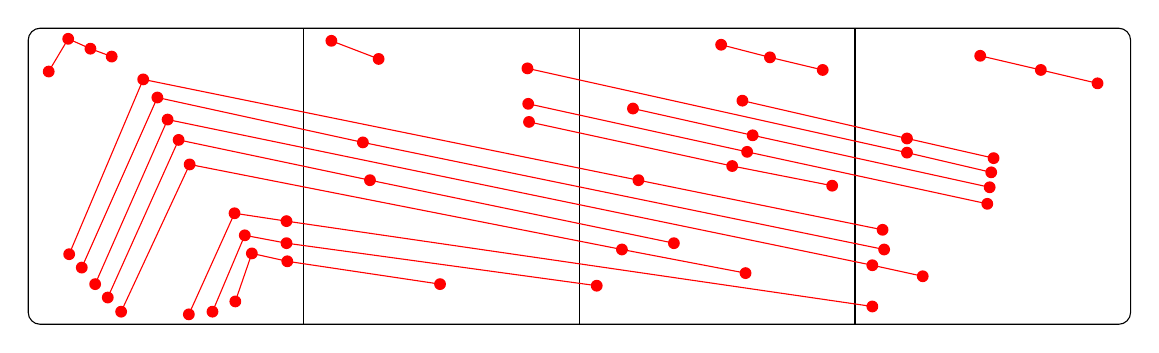
\begin{tikzpicture}[scale=1, every node/.style={scale=1}]
        \def\xscale{1.0} % Horizontal scale factor
        \def\yscale{1.0} % Vertical scale factor
        \def\spnt{0.075} % Size of smaller points
        \def\lpnt{0.125} % Size of larger points
        \def\roundscale{0.5} % The rounding factor
        \draw[rounded corners=2ex*\roundscale] (0,0) rectangle (14.0*\xscale,3.76*\yscale);
        \draw (3.5*\xscale, 3.76*\yscale) -- (3.5*\xscale, 0);
        \draw (7.0*\xscale, 3.76*\yscale) -- (7.0*\xscale, 0);
        \draw (10.5*\xscale, 3.76*\yscale) -- (10.5*\xscale, 0);
        \fill[red] (3.85*\xscale, 3.6*\yscale) circle (\spnt);
        \fill[red] (4.45*\xscale, 3.37*\yscale) circle (\spnt);
        \draw[red] (3.85*\xscale, 3.6*\yscale) -- (4.45*\xscale,3.37*\yscale);
        \fill[red] (6.36*\xscale, 2.57*\yscale) circle (\spnt);
        \fill[red] (8.94*\xscale, 2.01*\yscale) circle (\spnt);
        \fill[red] (10.21*\xscale, 1.76*\yscale) circle (\spnt);
        \draw[red] (6.36*\xscale, 2.57*\yscale) -- (8.94*\xscale,2.01*\yscale) -- (10.21*\xscale,1.76*\yscale);
        \fill[red] (6.35*\xscale, 2.8*\yscale) circle (\spnt);
        \fill[red] (9.13*\xscale, 2.19*\yscale) circle (\spnt);
        \fill[red] (12.18*\xscale, 1.53*\yscale) circle (\spnt);
        \draw[red] (6.35*\xscale, 2.8*\yscale) -- (9.13*\xscale,2.19*\yscale) -- (12.18*\xscale,1.53*\yscale);
        \fill[red] (6.34*\xscale, 3.25*\yscale) circle (\spnt);
        \fill[red] (11.16*\xscale, 2.18*\yscale) circle (\spnt);
        \fill[red] (12.23*\xscale, 1.93*\yscale) circle (\spnt);
        \draw[red] (6.34*\xscale, 3.25*\yscale) -- (11.16*\xscale,2.18*\yscale) -- (12.23*\xscale,1.93*\yscale);
        \fill[red] (8.8*\xscale, 3.55*\yscale) circle (\spnt);
        \fill[red] (9.42*\xscale, 3.39*\yscale) circle (\spnt);
        \fill[red] (10.09*\xscale, 3.23*\yscale) circle (\spnt);
        \draw[red] (8.8*\xscale, 3.55*\yscale) -- (9.42*\xscale,3.39*\yscale) -- (10.09*\xscale,3.23*\yscale);
        \fill[red] (7.68*\xscale, 2.74*\yscale) circle (\spnt);
        \fill[red] (9.2*\xscale, 2.4*\yscale) circle (\spnt);
        \fill[red] (12.21*\xscale, 1.74*\yscale) circle (\spnt);
        \draw[red] (7.68*\xscale, 2.74*\yscale) -- (9.2*\xscale,2.4*\yscale) -- (12.21*\xscale,1.74*\yscale);
        \fill[red] (9.07*\xscale, 2.84*\yscale) circle (\spnt);
        \fill[red] (11.16*\xscale, 2.36*\yscale) circle (\spnt);
        \fill[red] (12.26*\xscale, 2.11*\yscale) circle (\spnt);
        \draw[red] (9.07*\xscale, 2.84*\yscale) -- (11.16*\xscale,2.36*\yscale) -- (12.26*\xscale,2.11*\yscale);
        \fill[red] (12.09*\xscale, 3.41*\yscale) circle (\spnt);
        \fill[red] (12.86*\xscale, 3.23*\yscale) circle (\spnt);
        \fill[red] (13.58*\xscale, 3.06*\yscale) circle (\spnt);
        \draw[red] (12.09*\xscale, 3.41*\yscale) -- (12.86*\xscale,3.23*\yscale) -- (13.58*\xscale,3.06*\yscale);
        \fill[red] (0.26*\xscale, 3.21*\yscale) circle (\spnt);
        \fill[red] (0.5075971682687679*\xscale, 3.6255329896438315*\yscale) circle (\spnt);
        \fill[red] (0.79*\xscale, 3.5*\yscale) circle (\spnt);
        \fill[red] (1.06*\xscale, 3.4*\yscale) circle (\spnt);
        \draw[red] (0.26*\xscale, 3.21*\yscale) -- (0.5075971682687679*\xscale,3.6255329896438315*\yscale) -- (0.79*\xscale,3.5*\yscale) -- (1.06*\xscale,3.4*\yscale);
        \fill[red] (2.63*\xscale, 0.29*\yscale) circle (\spnt);
        \fill[red] (2.84*\xscale, 0.9*\yscale) circle (\spnt);
        \fill[red] (3.29*\xscale, 0.8*\yscale) circle (\spnt);
        \fill[red] (5.23*\xscale, 0.51*\yscale) circle (\spnt);
        \draw[red] (2.63*\xscale, 0.29*\yscale) -- (2.84*\xscale,0.9*\yscale) -- (3.29*\xscale,0.8*\yscale) -- (5.23*\xscale,0.51*\yscale);
        \fill[red] (2.34*\xscale, 0.16*\yscale) circle (\spnt);
        \fill[red] (2.75*\xscale, 1.13*\yscale) circle (\spnt);
        \fill[red] (3.28*\xscale, 1.03*\yscale) circle (\spnt);
        \fill[red] (7.22*\xscale, 0.49*\yscale) circle (\spnt);
        \draw[red] (2.34*\xscale, 0.16*\yscale) -- (2.75*\xscale,1.13*\yscale) -- (3.28*\xscale,1.03*\yscale) -- (7.22*\xscale,0.49*\yscale);
        \fill[red] (2.04*\xscale, 0.1261498920289589*\yscale) circle (\spnt);
        \fill[red] (2.62*\xscale, 1.41*\yscale) circle (\spnt);
        \fill[red] (3.28*\xscale, 1.31*\yscale) circle (\spnt);
        \fill[red] (10.72*\xscale, 0.2261498920289589*\yscale) circle (\spnt);
        \draw[red] (2.04*\xscale, 0.1261498920289589*\yscale) -- (2.62*\xscale,1.41*\yscale) -- (3.28*\xscale,1.31*\yscale) -- (10.72*\xscale,0.2261498920289589*\yscale);
        \fill[red] (1.01*\xscale, 0.34*\yscale) circle (\spnt);
        \fill[red] (1.91*\xscale, 2.3416773657739633*\yscale) circle (\spnt);
        \fill[red] (4.34*\xscale, 1.83*\yscale) circle (\spnt);
        \fill[red] (8.2*\xscale, 1.03*\yscale) circle (\spnt);
        \draw[red] (1.01*\xscale, 0.34*\yscale) -- (1.91*\xscale,2.3416773657739633*\yscale) -- (4.34*\xscale,1.83*\yscale) -- (8.2*\xscale,1.03*\yscale);
        \fill[red] (0.68*\xscale, 0.72*\yscale) circle (\spnt);
        \fill[red] (1.64*\xscale, 2.88*\yscale) circle (\spnt);
        \fill[red] (4.25*\xscale, 2.31*\yscale) circle (\spnt);
        \fill[red] (10.87*\xscale, 0.95*\yscale) circle (\spnt);
        \draw[red] (0.68*\xscale, 0.72*\yscale) -- (1.64*\xscale,2.88*\yscale) -- (4.25*\xscale,2.31*\yscale) -- (10.87*\xscale,0.95*\yscale);
        \fill[red] (1.18*\xscale, 0.16*\yscale) circle (\spnt);
        \fill[red] (2.05*\xscale, 2.03*\yscale) circle (\spnt);
        \fill[red] (7.54*\xscale, 0.95*\yscale) circle (\spnt);
        \fill[red] (9.11*\xscale, 0.65*\yscale) circle (\spnt);
        \draw[red] (1.18*\xscale, 0.16*\yscale) -- (2.05*\xscale,2.03*\yscale) -- (7.54*\xscale,0.95*\yscale) -- (9.11*\xscale,0.65*\yscale);
        \fill[red] (0.52*\xscale, 0.89*\yscale) circle (\spnt);
        \fill[red] (1.46*\xscale, 3.11*\yscale) circle (\spnt);
        \fill[red] (7.75*\xscale, 1.83*\yscale) circle (\spnt);
        \fill[red] (10.85*\xscale, 1.2*\yscale) circle (\spnt);
        \draw[red] (0.52*\xscale, 0.89*\yscale) -- (1.46*\xscale,3.11*\yscale) -- (7.75*\xscale,1.83*\yscale) -- (10.85*\xscale,1.2*\yscale);
        \fill[red] (0.85*\xscale, 0.51*\yscale) circle (\spnt);
        \fill[red] (1.77*\xscale, 2.6*\yscale) circle (\spnt);
        \fill[red] (10.72*\xscale, 0.75*\yscale) circle (\spnt);
        \fill[red] (11.36*\xscale, 0.61*\yscale) circle (\spnt);
        \draw[red] (0.85*\xscale, 0.51*\yscale) -- (1.77*\xscale,2.6*\yscale) -- (10.72*\xscale,0.75*\yscale) -- (11.36*\xscale,0.61*\yscale);
\end{tikzpicture}
\end{center}
    \caption{The pair of tilings that motivated the sliding strategy. The one above is the one encountered when mimicking the strategies of a specification for $\Av{1234}$ to a $\Av{1432}$ root while the one below is the one we needed to have identical specification in terms of strategies and structure.}
    \label{fig:slidepair}
\end{figure}

\section{Column reverse}
\input{chapters/03_1_crev}
\section{Column permutation}
\input{chapters/03_2_cperm}
\section{Sliding}
\input{chapters/03_3_slide}